% INTRODUCTION

% \todo[inline,color=yellow!40]{The introduction is one of the most important pieces of your thesis.  Here is a place for you to introduce the problem(s) on which you have worked and place them in the larger context of your field. You should aim to ensure that this section is completely understandable to virtually anyone - and certainly anyone with a sophomore-level grasp of physics.  Presumably, this will include references to the literature.
% \\
% In addition to setting your work into context, a second good idea for your introduction is to give a short outline for what the rest of your thesis will discuss.  This is often done in the closing paragraph(s) of the introduction with sentences like ``In the following chapters \ldots " and ``Chapter 2 discusses \ldots"  Tremendous detail is not required in this outline, but rather just a brief road map for the rest of the document.}

Synchrotron radiation was first observed by General Electric in Schenectady, New York \cite{firstSynchrotronRadPaper}. Initially just a side effect of particle accelerator experiments, it has since grown to be an important and powerful source of high-energy electromagnetic radiation for structural determination. Compared to lab-scale x-ray generation for diffraction experiments, arguably the most important benefit of synchrotron radiation is its high brilliance. Synchrotron radiation creates a highly collimated beam of photons characterized by small divergence and spatial coherence. Additionally, synchrotron radiation is tunable across a wide spectrum (microwaves to hard X-rays) and capable of high flux, useful for short time-scale-dependent experiments or weak scatterers. Synchrotron radiation can be produced in a pulsed structure. Importantly, the incoming photons are highly polarized, either linearly or circularly, depending on where the measurement system lies with respect to the plane of the synchrotron. The advent of a technique to manufacture such a high-quality source of x-rays allowed for new, advanced methods of x-ray absorption spectroscopy, and the two fields were developed in parallel \cite{synchrotronbook}. 

\section{X-ray Absorption Spectroscopy}
X-ray absorption spectroscopy (XAS) measures the absorption of high-energy photons by a sample as a function of energy \cite{gardenghi2012synchrotron}. X-ray Absorption Fine-Structure (XAFS) spectroscopy refers to the study of absorption spectra created from high-intensity x-ray interactions. An incident photon is only absorbed by a bound electron in cases where the photon's initial energy is at least as great as the energy difference between the electron’s initial quantum state and the next allowed quantum state (or unoccupied continuum level) \cite{einstein1905photoelectriceffect}. The attenuation, or change in transmitted light intensity as a result of inelastic processes, is characterized by the Beer-Lambert Law (\ref{BeerLambert}). For an incident beam of intensity $I_0$, the transmitted intensity after interacting with an attenuation
coefficient of $ \mu $ and a sample of thickness $ x $ is: 

\begin{equation}
    \label{BeerLambert}
    I_t = I_0 e^{-\mu x}
\end{equation}

For x-rays (.5--50~keV), absorption of the incident photon by core-level electrons is possible. At this energy, nearly all the photon's energy is absorbed by the core electron, resulting in the characteristic absorption-edges first observed in 1920 \cite{fricke1920, hertz1920ueber}. When an x-ray with energy greater than the binding energy of a core level electron is absorbed, the electron is “ejected” (i.e., “excited”) and imparted with the excess energy in the form of momentum. Electrons ejected in this manner are referred to as ``photoelectrons'' or electrons in an excited state, and result in a ``core-hole'' at the core level of the electronic shell. This core-hole is filled either by a an electron in a higher level and the emission of an Auger electron or fluroescence. In either case, the original excited electron decays rapidly---on the order of femptoseconds---and leads to the emergence of a ``fine structure'' in the absorption vs. incident photon energy plot. As the energy of the incident radiation increases, the photon's energy will eventually match the binding energy of a core-level electron. As a result, an ``edge'' in the spectrum will be observed. The location of these edges depends on the chemical and physical structure, as well as the electronic and vibrational states of the material. Absorption edges are like fingerprints used to identify elements, distinguish oxidation states, and even probe short-range order from the characteristic peaks and oscillations in the spectrum. XAFS spectroscopy can be performed on virtually any stable element since all atoms contain core-level electrons. Although a high-quality source of x-rays such as synchrotron radiation is required for the analysis, the ubiquity and utility of XAFS spectroscopy has made it an indispensable technique in fields such as materials biology, chemistry, and materials science \cite{rehrXAFS2000review} \cite{newville2014fundamentals}.

In experimental setups, particular energy photons are selected from the broad spectrum of synchrotron radiation via a pair of monochromators. The primary monochromator is a crystal with interplanar spacing ($ d $) chosen specify to satisfy the Bragg equation \ref{Bragg}, reflecting photons of wavelength, $ \lambda $ at angle $ \theta $.  

\begin{equation}
    \label{Bragg}
    n\lambda = 2d\sin(\theta)
\end{equation}

The secondary monochromator removes higher-order harmonics that satisfy the Bragg equation $ (2\lambda,~3\lambda~etc.). $ Different wavelengths of light are selected by changing the angle. A common method for XAFS analysis involves scanning the monochromators over an energy range. In the XAFS setup, two ionization chambers are used to measure the incident and transmitted light intensity. For any experiment, the absorption spectrum for a reference sample is also measured to calibrate the energy scale \cite{exafsxanes1988}. A diagram depicting a simplified experimental setup for an XAFS experiment is presented in Figure \ref{fig:xafs-setup}.  

\begin{figure}[h]
    \centering
    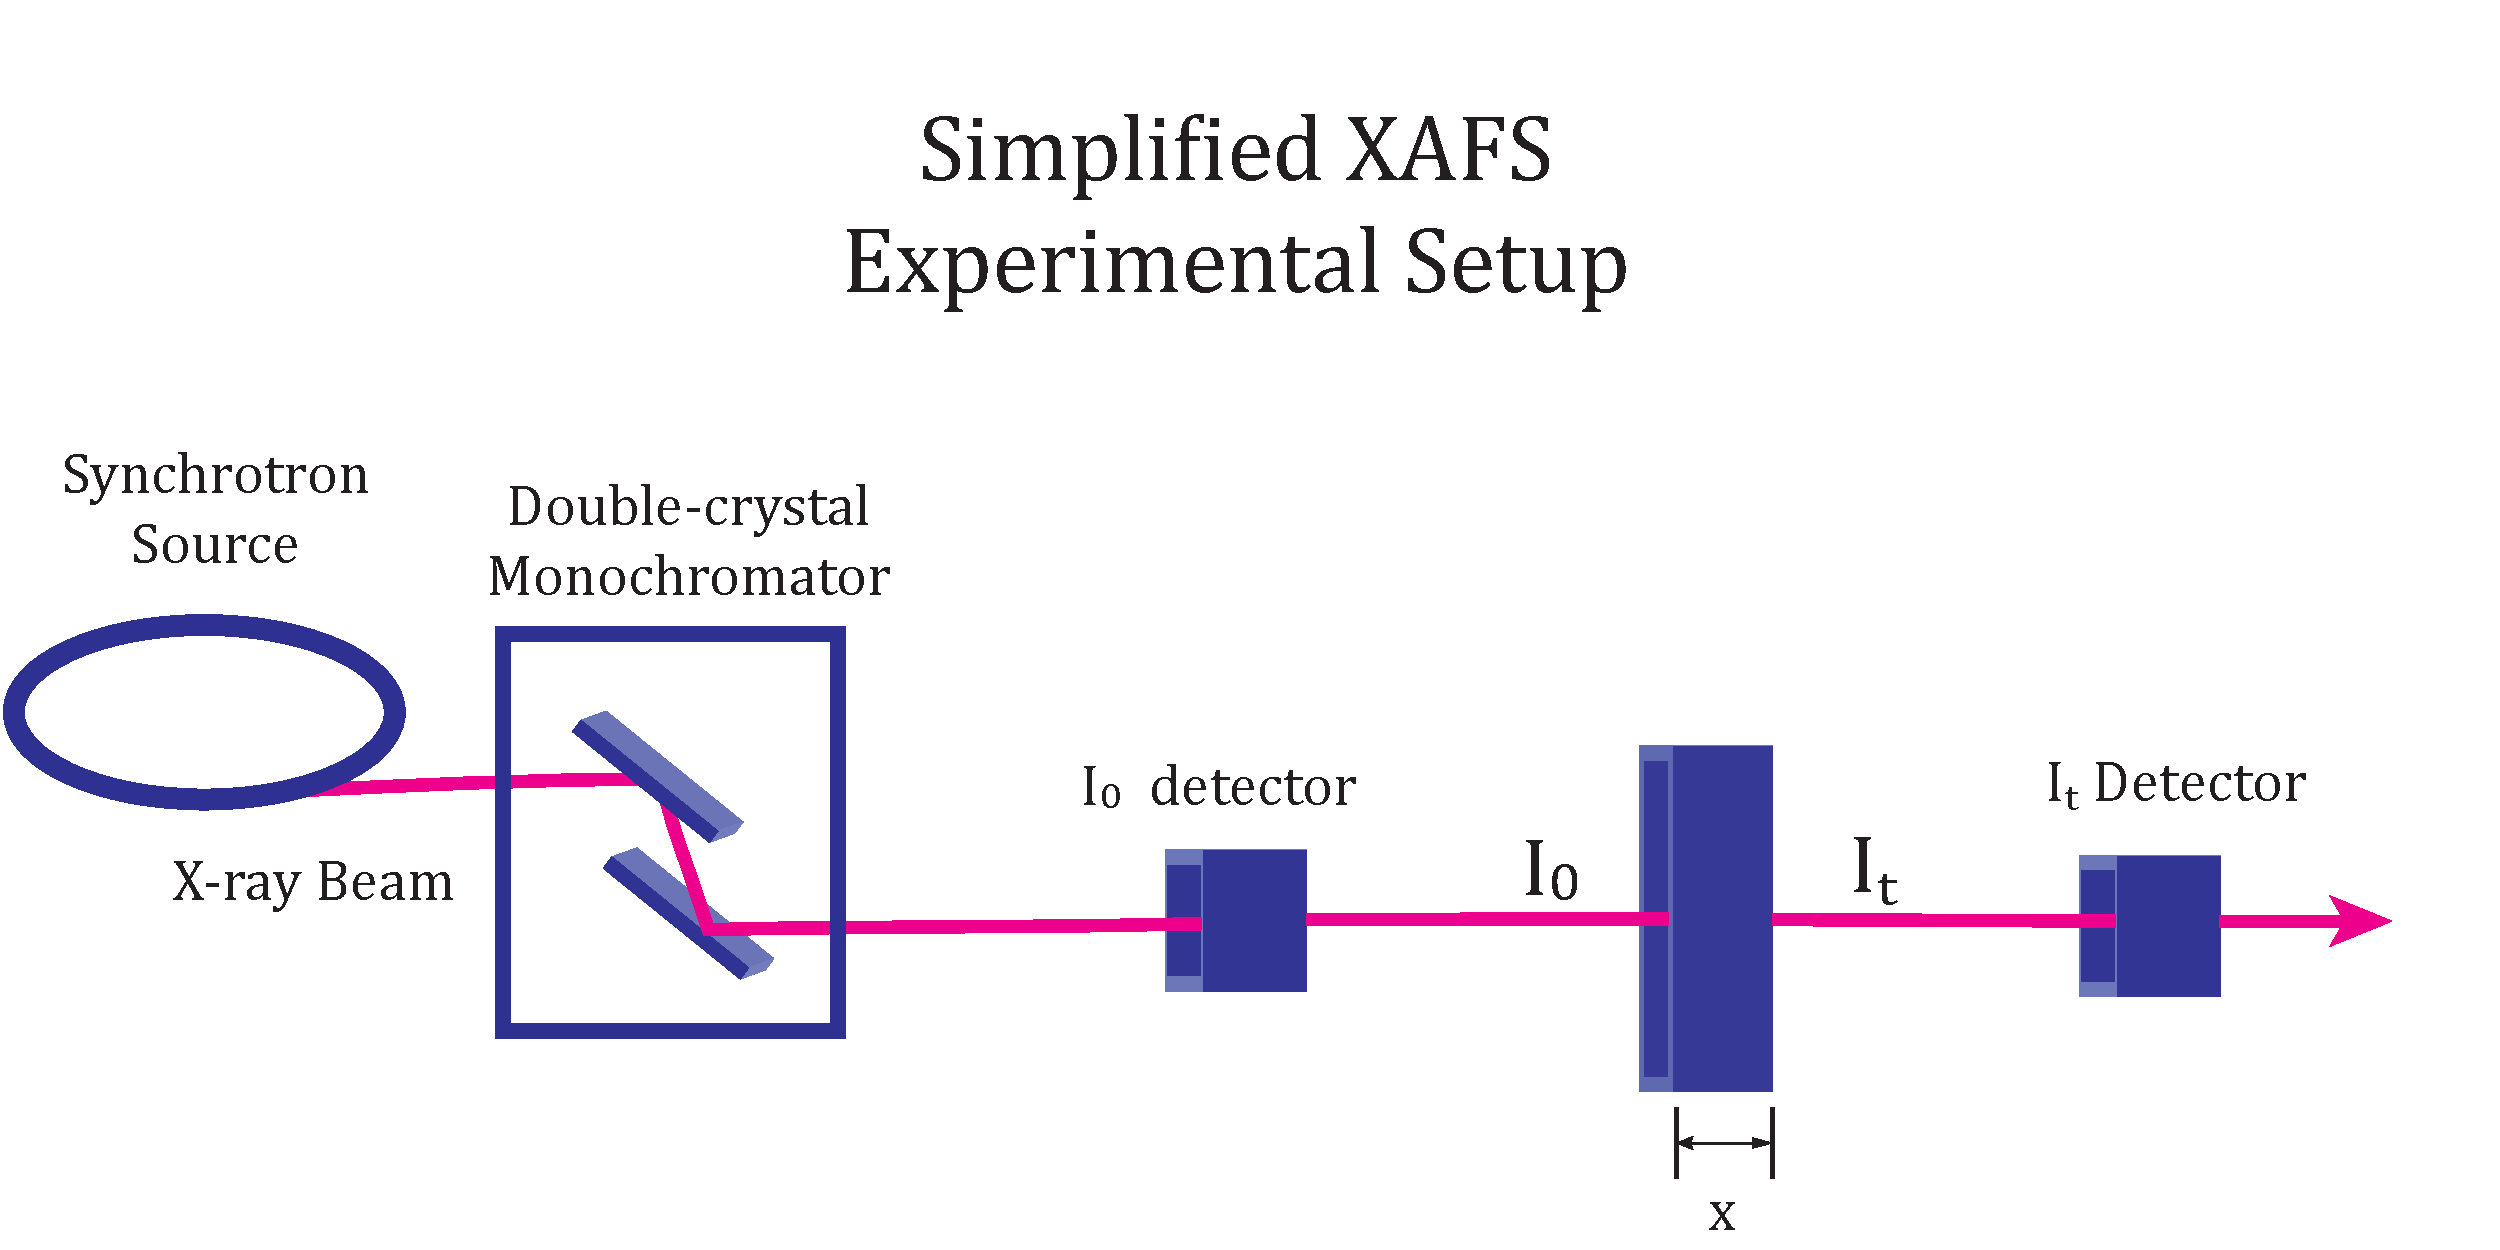
\includegraphics[width=\linewidth]{Chapters/Figures/synchrotron-diagram.pdf}
    \caption[Example XAFS Experiment Setup]{A simplified diagram for an x-ray absorption spectroscopy experiment. The high brilliance x-rays are produced from the synchrotron and then collimated through a monochromator. The beam is then split, with one half sent to an ionization chamber to measure the initial x-ray intensity, $ I_0 $ . The other half is sent towards the sample, where a second ionization chamber awaits the beam on the other side to measure the intensity of the transmitted beam, $ I_t $.}
    \label{fig:xafs-setup}
\end{figure}

% \subsection{XAFS}
% X-ray Absorption Fine-Structure (XAFS) spectroscopy refers to the study of absorption spectra created from high-intensity x-ray interactions. As the energy of the incident radiation increases, the photon's energy will eventually match the binding energy of a core-level electron. As a result, an ``edge'' in the spectrum will be observed. The location of these edges depends on the chemical and physical structure, as well as the electronic and vibrational states of the material. Absorption edges are like fingerprints used to identify elements, distinguish oxidation states, and even probe short-range order from the characteristic peaks and oscillations in the spectrum. XAFS spectroscopy can be performed on virtually any stable element since all atoms contain core-level electrons. Although a high-quality source of x-rays such as synchrotron radiation is required for the analysis, the ubiquity and utility of XAFS spectroscopy has made it an indispensable technique in fields such as materials biology, chemistry, and materials science \cite{rehrXAFS2000review} \cite{newville2014fundamentals}.

% The XAFS equation is: 
% \begin{equation}
%     \label{XAFS}
%     \chi = \dfrac{ \mu(E)- \mu_{0}(E)  }{  \mu_{0}(E) - \mu_{ b  }(E)  } 
% \end{equation}

% \noindent where $\mu$ is the measured absorption, $ \mu_0 $  is the ``atomic'' absorption due to .... specific electrons, and $ \mu_b $ 
% is the absorption of other processes \cite{klementev2000xafs}, typically approximated with the Victoreen polynomial (\ref{Victoreen}).

An example XAFS spectrum is plotted in Figure \ref{fig:Unnormalized-XAFS}. The overall shape of the spectra is characterized by a large jump followed by oscillations. The absorption steadily decreases as a function of increasing energy. The slope of this decrease is often approximated by the Victoreen formula (\ref{eqn:Victoreen}. 

\begin{equation}
    \label{eqn:Victoreen}
    \mu_b(E) = aE^{-3} + bE^{-4}
\end{equation}

\noindent The coefficients $ \alpha $ and $ \beta $ can be found via a simple regression on a sprectrum measured at pre-edge energies \cite{klementev2000xafs}.Typically XAFS spectra are normalized to affix the decaying absorption beyond the first edge to a value of one (See Figure \ref{XAFS-example-spectrum}). The large jump in absorption is referred to as the "edge" and caused by the sudden complete absorption of X-rays by electrons at the core binding energy. New edges are intrduced when the incident energy matches the binding energy of a different energy electron. Each edge is labeled according to the quantum numbers: the K-edge corresponds to the 1s level, L1 to the 2s level, and L2 and L3 refer to the relativistically-split $ P_{1/2} $  and $ P_{3/2} $ level. This degeneracy causes the L3 absorption edge to have a greater edge jump than L1 or L2 \cite{absorptionSpecArticle}. Regions far from the edge are relatively smooth and caused by the background absorption of x-rays. At energies beyond the edge, the absorption spectrum is characterized by oscillations referred to as the fine structure.

The XAFS spectrum is typically divided into two regions of study: the area near the first absorption peak (XANES) and the area after (EXAFS). XANES has a strong sensitivity to the oxidation state and coordination chemistry of the absorbing atom, while the EXAFS can be used to determine the bond lengths, coordination numbers, and atomic species of the absorbing atom's neighbors.

\begin{figure}
    \centering
    \includegraphics[width=.75\linewidth]{Chapters/Figures/un-normalized-xafs.png}
    \caption{Unnormalized spectrum from Nick. Need to fix this. Info about it on page 30/49 of Nick's dissertation.}
    \label{fig:Unnormalized-XAFS}
\end{figure}

\begin{figure}
    \centering
    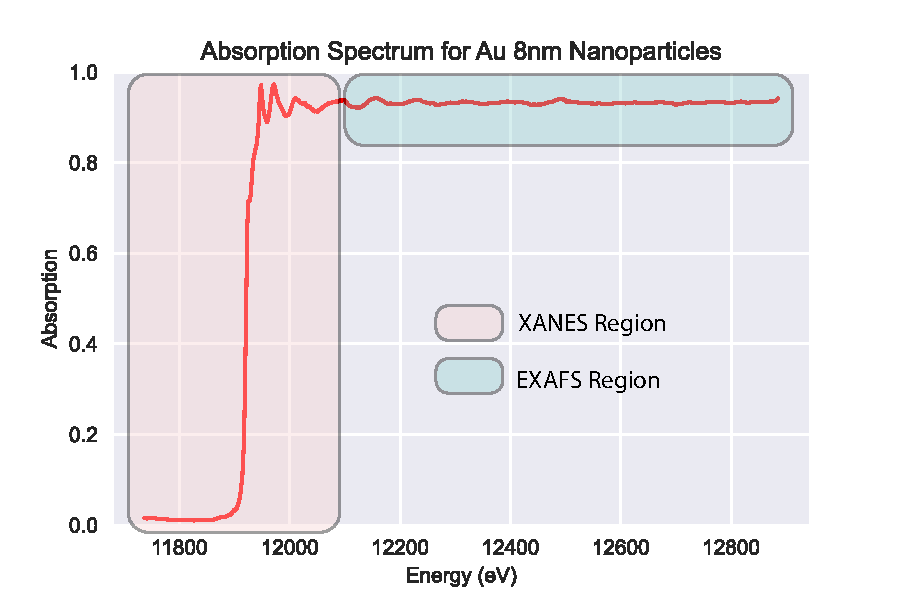
\includegraphics[width=.75\linewidth]{Chapters/Figures/absorption-spectra-example.pdf}
    \caption{The absorption spectrum is divided into two regions: XANES and EXAFS. The XANES (x-ray absorption near edge structure) includes the lower energy region in the direct vicinity of the leading edge. The EXAFS (extended x-ray absorption fine structure) region includes all the energies beyond the XANES.}
    \label{XAFS-example-spectrum}
\end{figure}
% "The most difficult procedure in extracting of XAFS from the measured absorption is the construction of μ0 since
% one cannot definitely distinguish the environmental-born part of absorption from the atomic-like one. \cite{klementev2000xafs}"

\subsection{EXAFS}
Beginning approximately 50~eV beyond the edge of the absorption spectrum lies the Extended X-ray Absorption Fine Structure (EXAFS) region. The spectral shape of this domain is determined by the multiple scattering of the photoelectron, interference of the incoming and outgoing waves of the photon, and electronic energy level splitting of the local structure. The oscillations in the EXAFS region are extremely sensitive to local bond lengths, coordination numbers, and atomic species of the surrounding elements.

The EXAFS fine structure is the product of the photoelectrons' self-interference as they are scattered by the local atomic environment surrounding the absorbing atoms from which they were excited.

\subsubsection{EXAFS Data Reduction}
Preparing the absorption data for fitting requires series of steps in preparation. These preparation steps are known as data reduction. First, the pre-edge background must be removed using the Victoreen formula (\ref{eqn:Victoreen}) or an alternative polynomial. Next, the atomic background, $ \mu_0(E) $  is removed, and the absorption measured absorption is normalized accordingly. This is a non-trivial process, as the absorption coefficient is not that of a single, isolated atomic absorber; instead, it represents that of an atom and its surrounding neighbors. High-order spline fittings must be used to remove the low-frequency, immeasurable oscillations caused by photoelectron scattering with nearby valence electrons. For EXAFS Fitting, the EXAFS function is often transformed into k-space, and Fourier transformed into a radial distribution-like function via (\ref{rdf-exafs}) \cite{exafsbook}.

\begin{equation}
    \label{rdf-exafs}
    \widetilde{\chi}(r) = \frac{1}{2\pi} \int_{0}^{\infty }  k^n \chi(k) e^{2ikr} dk
\end{equation}

Alternatively, one can convert the wave to R-space. Two of the most popular EXAFS fitting programs, Artemis and Athena, convert to R-space.

\subsubsection{The EXAFS Equation}
With the data reduction complete, a multi-parameter fitting can be performed via the {EXAFS} equation. This equation is an approximation based principally on the single electron approximation of Fermi golden rule (\ref{FermisGoldenRule}).

\begin{equation}
    \label{FermisGoldenRule}
    % Fermi's GOlden Rule for a one e- approximation
    \mu(\omega) \varpropto  \sum_{f}^{E_f > E_F} \left\langle \psi_i \lvert \Delta \rvert \psi_f \right\rangle ^2 \delta (E_F - E_i - \hbar \omega)  
\end{equation}

% \begin{equation}
%     \label{FermisGoldenRule}
%     % Fermi's GOlden Rule for a one e- approximation
%     \mu(E) \varpropto \sum_{f}^{E_f > E_F} \left\lvert \left\langle f \lvert H_{int} \rvert i \right\rangle \right\rvert ^2 \delta (E - E_F - E_f)  
% \end{equation}
% $ H_{int} $ is the matter-light interaction operator,

\noindent Fermi's golden rule describes the probability of a transition in state occurring. Here (\ref{FermisGoldenRule}), $ \mu(\omega) $ is the absorption coefficient, $ f $ and $ i $ are the final and initial eigenstates of the photoelectron, respectively, $ \Delta $ is the dipole transition operator, and the delta function $ \delta $ ensures conservation of energy. The transition operator $ \Delta $ represents the interaction between the electrons and photon and is constrained by the dipole approximation. The constructive and descructive interference of the outgoing and backscattered waves modulates the transition matrix element coupling coupling the initial nad final states, resulting in the fine structure in XAS. The summation of all energy values approximates the many-bodied problem as a single particle theory. 

At energies above the core electron binding energy, excess energy is transferred to the photoelectron, which may then undergo multiple scattering with the surrounding atoms. The final wavefunction of the photoelectron is the superposition of the outgoing photoelectron and the scattered wave \cite{anotherxafstocite}. EXAFS only takes into account the local region around the absorber at a distance $ r_j $  from the backscattering atom. The absorption coefficient, $ \mu $, is proportional to the transition rate given by Fermi’s golden rule. Therefore,  $ \mu $ depends on the energy and symmetry of both the initial and final electron states \cite{xafsXanesFermisGoldenRule}. 

% The EXAFS signal for one backscattering atom can be described as (\ref{superposition_Exafs}). 
% \begin{equation}
%     \label{superposition_Exafs}
%     \chi(k) \approx F_j(k) \dfrac{\sin[2kr_j + \phi_{ij}(k)]}{2r_j^2}
% \end{equation}

For a system with multiple atoms, one must sum over all the backscattered waves. The total EXAFS signal is the sum of all possible photoelectron scattering paths; this includes both single scattering and multiple scattering. The summation over all single scattering paths in the first nearest-neighbor shell can be written as: \textit{(135, 136):}

\begin{equation}
    \label{first-nn-exafs-single-scattering}
    \chi(k) = \sum_i S_0^2 \int_{0}^{\infty} g_i(R) f_i(k, R) e^{-2R/\lambda(k)} \sin[2kR + \phi_i(k, R)]  \,\frac{dR}{kR^2} 
\end{equation}

\noindent where $ \chi $ is the total strength of the EXAFS signal and $ S_0$ is an amplitude correction factor. Here (\ref{first-nn-exafs-single-scattering}), $g_i(R)$ is the radial distribution function (RDF). The terms $ S_0^2 $, $ f_i (k, R) $, $\lambda(k)$, and $\phi_i(k, R)$ are related to the local structure described by the RDF and material specific. They are determined by factors such as interatomic distances, degree of structural disorder, and the number of nearest neighbors.

To account for the inevitable variation in bond lengths, the Debye-Waller factor $ \sigma_j $ is introduced; $ \sigma_j $ describes the standard deviation of bond-lengths of the sample.\footnote{Note, this differs from the Debye-Waller factor used for x-ray absorption, which describes the broadening of a diffraction peak due to variations in inter-planar spacing \cite{DW-diffraction}}. The lifetime of the photoelectron's excited state is taken into account by introducing an exponential term to account for the mean-free-path, $ \text{exp}({-2r_j/\lambda}) $. Combining all this information, we arrive at the EXAFS equation (\ref{ExafsFormula}). 

\begin{equation}
    \label{ExafsFormula}
    \chi(k) = \sum_j \frac{N_j}{kr_j^2}F_j(k)\text{exp}({-2\sigma_j^2k^2})\text{exp}({-\tfrac{2r_j}{\lambda(k)}})\sin[2kr_j + \phi_{ij}(k)]
\end{equation}

\noindent

To recapitulate all the terms in (\ref{ExafsFormula}): $ N_j  $ is the coordination number of atom j; $ k $  is the wavenumber; $ r_j $ is the distance to neighboring atom $ j $;$ F_j(k) $  is a scattering property of the neighboring atoms; $ \text{exp}({-2\sigma_j^2k^2}) $ is an exponential dampening term dependent on the variance in bond length $ \sigma_j^2 $; $ \phi_{ij} $ includes the phase shifts for the incoming and outgoing waves and  accounts for scatting off non-point-like atoms.    

Although popular, the EXAFS equation is still a first-order approximation with assumptions and limitations. For example, the fitted disorder parameter, the Debye-Waller factor, explicitly assumes a Gaussian distribution of nearest-neighbor bond length distances. Other more accurate but computationally intensive alternatives are increasing in popularity. Such alternatives include molecular dynamics \cite{mol-dyn-xanes}, reverse Monte Carlo simulations \cite{RMC-xanes} and neural networks \cite{lin2020machine} \cite{timoshenko2018neural}.

\subsection{XANES}
The XANES region, or the near-edge region, encodes the chemical and electronic structural information of the sample within its shape. The XANES shape reflects the lower energy photons that scatter much more strongly than in the EXAFS region. XANES also has the advantage of a higher signal-to-noise ratio than the subtle interference-determined oscillations found in EXAFS. While there is an ``EXAFS Equation,'' there is no ``XANES Equation'' equivalent; however, this does not mean that there is no structural information encoded in the XANES, only that the theory is underdeveloped. Mainly, the strong errors in potential and many-body effects limit the development of a ``XANES equation.'' 

With the recent explosion in the popularity of machine learning, the investigation of the XANES latent space has become a topic of modern research is. In other words, \textit{how much information is encoded in XANES?}

Recent work at Brookhaven National Laboratory \cite{Timoshenko2017} has shown that a model can learn structural descriptors from the XANES spectrum. Specifically, their method enables the decoding of XANES spectra to obtain the coordination number of metallic nanoparticles. In this 2017 paper, the group trained an artificial neural network (ANN) to recognize a relationship between the nanoparticle structure and the XANES spectrum. Once trained, the ANN is used to ``invert'' an unknown spectrum to obtain the corresponding structural descriptors of the catalyst. These descriptors, the coordination numbers, are used to calculate the number of shells (nanoparticle size) and shape (Archimedian solid) of the sample. While this model can determine the structure of nanoparticles from XANES ---a feat previously only possible with the full EXAFS spectrum ---it still has one major limitation: the ANN does not predict the disorder of the structure. The bond-length disorder is known to be an important descriptor for catalyst \cite{catalyst-strain-dependence} \cite{co-strain-effects}.

\begin{figure}
    \centering
    \includegraphics[width=.75\linewidth]{Chapters/Figures/placeholderFrenkel2017.png}
    \caption[ANN Metallic Nanoparticles]{From \cite{Timoshenko2017}, the neural netowrk is trained to take a XANES spectrum from a metallic nanoparticle, and predict the coordination number of the structure. This coordination number of nanoparticles is a known discriptor, which allows for easy calculation of the the nanoparticle's size and shape.}
\end{figure}

\section{Goals of the Thesis and Approach}
Building on the previous work \cite{Timoshenko2017}, the goal of this thesis is comprised of two parts. First, we seek to determine whether bond-length information is encoded in the XANES spectrum. Second, we utilize machine learning to predict the bond-length (static) disorder from a XANES spectrum. As with the 2017 BNL paper \cite{Timoshenko2017}, the work in this thesis was conducted with gold (Au) due to the availability of relevant experimental data. While an ongoing goal is to expand this thesis' work to Au nanoparticles (among other elements), we primarily choose to simulate bulk Au to mitigate additional complexity driven by surface effects. Machine learning requires a substantial amount of training data, far more than could be experimentally obtained. Instead, we rely on absorption simulation software to create the training data: a collection of XANES spectra for large, bulk-like Au nanoparticles with known disorders. The network is then trained on the theoretical XANES spectra. Because of the systematic differences between the simulation and experimental data, the network must then be adjusted in order to be able to predict experimental data.

\section{Outline of the Thesis}
Often, the most time-intensive part of a machine learning-based project is the process of collecting and preprocessing the data. Chapter 2 is dedicated entirely to the process of generating XANES spectra via simulations. Next, a solid foundational understanding of machine learning is integral in understanding the approach. All the machine learning terms present in later chapters are defined here.  Chapter 4 describes the specif1ic model architecture and results of the training process. Further discussion and comments on future work are included in chapter 5. Appendix A includes a description of the main Python scripts written for this thesis, which are necessary for replicating the work. The file structure and some individual functions are included to clarify the calculation or creation of selected parameters and files. The files and scripts are available upon request by contacting the author.
% Building off the historical context of measuring disordered nanoparticles in XANES spectra, this thesis begins with an in-depth description of 
